%======================================================================
% poznamky_9_matice_hustoty.pdf
%======================================================================
\section{Kvantová statistika -- smíšené stavy, matice hustoty}
\strana{$\rho$1}

\underline{Motivace:} měření veličiny $\hat A$ ve stavu $\ket{\psi}$

\begin{tabular}{@{}lll@{\qquad}ll}
$\to$ nalezneme & $a_1$ \dots\ s pravd.\ $|\braket{a_1}{\psi}|^2$ & & stav po měření $\ket{a_1}$ s pravd.\ $p_1$ \\
 & $a_2$ \dots & $p_2 = |\braket{a_2}{\psi}|^2$ & \quad --\,{\textquotedbl}\,-- \quad $\ket{a_2}$ \quad --\,{\textquotedbl}\,-- \quad $p_2$ \\
 & \ \vdots & \ \vdots & \hspace{2.6cm}\vdots
\end{tabular}

Popis dalšího vývoje / měření v systému?

\kw{statistický soubor} \quad $\{\ket{\psi_i}, p_i\}_{i=1}^N$ \quad \dots\ předp.\ $\ket{\psi_i}$ normované a $\sum p_i = 1$ \\
\hspace*{7.6cm} (ne nutně ortogonální)

Další měření např.\ veličiny $\hat B$ \\
\quad $\to$ nalezení $b_1$ s pravd.\ \quad $\sum_i p_i\,|\braket{b_1}{\psi_i}|^2 = p_{b_1}$ \quad \dots\ součet podmíněných pravděpodobností!

a například \quad $\langle\hat B\rangle = \sum_i p_i\mel{\psi_i}{\hat B}{\psi_i}$
\quad \pozn{$\equiv \sum_b \bra{b}\hat B\sum_i\ket{\psi_i}p_i\bra{\psi_i}\ket{b}$}

Při dalším měření se změní statistický soubor a může se měnit i počet jeho prvků.

\begin{definice}[Matice hustoty]
Elegantní popis $\to$ \kw{Matice hustoty} (statistický operátor)
\[
  \vzorec{\hat\rho \equiv \sum_{i=1}^N p_i\ket{\psi_i}\bra{\psi_i}}
\]
\end{definice}

\hfill\textcolor{Red}{Ballentine \dots\ prostě \uv{stav} \(\downarrow\)}

\begin{tabular}[t]{@{}l|}
\underline{výhoda:} bez ohledu na $N$ vždy operátor v $\mathcal{H}$ (matice $\dim\mathcal{H}\times\dim\mathcal{H}$) \\
\pozor{!} každé měření lze popsat pomocí $\hat\rho$ \\
\phantom{!} dva statistické soubory popsané stejným $\hat\rho$ jsou nerozlišitelné žádným měřením
\end{tabular}

\subsection*{Měření}
\begin{itemize}
  \item normování $\rho$: \quad $\vzorec{\operatorname{Tr}\rho = 1}$ \quad (odpovídá $\sum_n p_n = 1$) \\
        \pozn{DK: $\operatorname{Tr}\rho \equiv \sum_{\ket{m}}\sum_i p_i\braket{m}{\psi_i}\braket{\psi_i}{m} = \sum_i p_i\braket{\psi_i}{\psi_i} = \sum p_i = 1$}
\end{itemize}

\noindent\rule{\linewidth}{0.4pt}

\underline{Vsuvka:} \quad STOPA OPERÁTORU \quad nechť $\{\ket{m}\}$ je ON báze v $\mathcal{H}$.

\begin{definice}[Stopa operátoru]
Pak \quad $\operatorname{Tr}\rho \equiv \sum_m\mel{m}{\rho}{m}$ \hfill (ve funkcionální analýze důležitá třída operátorů $\operatorname{Tr}\rho < \infty$)
\end{definice}

\begin{itemize}[label=--]
  \item stopa nezávisí na bázi
  \[
    \operatorname{Tr}_{\tilde m}\rho \equiv \sum_{\tilde m}\bra{\tilde m}\underset{I}{\vphantom{\big|}}\rho\underset{I}{\vphantom{\big|}}\ket{\tilde m}
    = \sum_{m'm''\tilde m}\underbrace{\braket{\tilde m}{m'}\mel{m'}{\rho}{m''}\braket{m''}{\tilde m}}_{\text{matice přechodu unit.} \,\to\, \delta_{m'm''}}
    = \sum_{m'm''}\delta_{m'm''}\mel{m'}{\rho}{m''} \qquad\text{c.b.d.}
  \]
  \item cyklická vlastnost stopy: \quad ($A, B$ operátory)
  \[
    \vzorec{\operatorname{Tr}\{AB\} = \sum_{mn}\mel{m}{A}{n}\mel{n}{B}{m} = \sum_{mn}\mel{n}{B}{m}\mel{m}{A}{n} = \operatorname{Tr}\{BA\}}
  \]
\end{itemize}

\noindent\rule{\linewidth}{0.4pt}

poznámka: někdy se pracuje s nenormovanou $\hat\rho$ \dots\ to lépe vystihuje jeden válec s celkovou pravděpodobností $p = \operatorname{Tr}\hat\rho$

%----------------------------------------------------------------------
\strana{$\rho$2}
\subsection*{Měření}
\begin{itemize}
  \item střední hodnota operátoru $\hat A$: \quad $\vzorec{\langle A\rangle = \operatorname{Tr}\{\rho A\}}$ \\
        \pozn{$\langle A\rangle = \sum_i p_i\mel{\psi_i}{A}{\psi_i} = \sum_{im}p_i\braket{\psi_i}{m}\mel{m}{A}{\psi_i} = \sum_m\bra{m}A\underbrace{\Big(\textstyle\sum_i\ket{\psi_i}\bra{\psi_i}p_i\Big)}_{\rho}\ket{m}$}
  \item pravděpodobnost nalezení systému ve stavu $\ket{\phi}$
  \[
    p_\phi = \mel{\phi}{\rho}{\phi} = \operatorname{Tr}\{\rho\ket{\phi}\bra{\phi}\} = \operatorname{Tr}\{\rho P_\phi\} = \operatorname{Tr}\{P_\phi\rho P_\phi\}
    \quad \textcolor{Red}{\leftarrow}
  \]
  \item platí i pro pravd.\ nalezení jednoho ze stavů $\ket{\phi_i}$, mezi nimiž nemáme schopnost rozlišit \\
        $P \equiv \sum_i\ket{\phi_i}\bra{\phi_i}$ \quad ($\phi_i$ ON-množina) \hfill \textcolor{Red}{(viz $\uparrow$)}
        \begin{itemize}[label=--]
          \item stav po měření \quad $\tilde\rho = \dfrac{P\rho P}{\operatorname{Tr}\{P\rho P\}}$ \quad $\swarrow$ normování
        \end{itemize}
  \item stav po měření odp.\ operátoru $\hat A = \sum_a a\hat P_a$, tedy je
  \[
    \vzorec{\tilde\rho = \sum_a\frac{\hat P_a\hat\rho\hat P_a}{\operatorname{Tr}\{P_a\rho P_a\}}\,\mu_a = \sum_a\hat P_a\rho\hat P_a}
  \]
\end{itemize}

\underline{pozn:} pokud není $\hat\rho$ normovaná, je třeba ve vzorcích pro pravděpodobnost nahradit $\hat\rho\to\dfrac{\hat\rho}{\operatorname{Tr}\hat\rho}$; nebo chápat výsledek jako podmíněnou pravděpodobnost.

\subsection*{Vlastnosti $\hat\rho$}
\begin{veta}[Vlastnosti matice hustoty]
\begin{itemize}
  \item evidentně \quad $\hat\rho^\dagger = \hat\rho$ \quad ($p_i\in\mathbb{R}$) \hfill \kw{Hermitovskost}
  \item $\mel{u}{\hat\rho}{u} \geq 0 \quad \forall\ket{u}$ \quad ($p_i\geq 0$) \hfill \kw{Pozitivní definitnost}
  \item spektrum: \quad $\hookrightarrow\ \Rightarrow$ \ $\forall$ vl.\ č.\ $\in\langle 0,1\rangle$ \ a vl.\ v.\ jsou ON množina (nebo lze volit) \\
        \pozn{pozn: připomínám, že původně mohlo být $\braket{\psi_i}{\psi_j}\neq 0$} \quad \textcolor{Red}{(pro normovanou $\operatorname{Tr}\rho = 1$)}
  \item platí \quad $\operatorname{Tr}\rho^2\in\langle 0,1\rangle$ \\
        přičemž \quad $\operatorname{Tr}\rho^2 = 1 \ \Leftrightarrow\ \rho = \ket{\psi}\bra{\psi}$ \quad \dots\ \kw{čistý stav}, \kw{polarizovaný} \\
        \hspace*{5.4cm} (koherentní směs $\ket{\psi} = \ket{\phi_1} + \ket{\phi_2}$) \\
        \phantom{přičemž} \quad $\operatorname{Tr}\rho^2 < 1$ \quad \dots\ \kw{nekoherentní}, \kw{smíšený stav}
\end{itemize}
\end{veta}

\subsection*{Časový vývoj}
Ve Schrödingerově reprezentaci:
\[
  i\hbar\pdv{t}\ket{\psi} = H\ket{\psi} \quad\Rightarrow\quad -i\hbar\pdv{t}\bra{\psi} = \bra{\psi}H
\]
\[
  \Rightarrow\quad \vzorec{i\hbar\pdv{t}\rho = [H,\rho]}
  \qquad\text{\dots\ \pozor{pozor} \dots\ obrácené znaménko než pro operátory v Heisenberg.\ obrázku}
\]
\underline{DK:} \quad $\hookrightarrow\ \sum_i\Big(\Big[i\hbar\pdv{t}\ket{\psi_i}\Big]p_i\bra{\psi_i} + \ket{\psi_i}p_i\pdv{t}\bra{\psi_i}\,i\hbar\Big) = H\rho - \rho H$

tj.\ čas.\ \sout{vývoj H}: \quad \fbox{$\rho(t) = e^{-\frac{i}{\hbar}Ht}\rho\,e^{\frac{i}{\hbar}Ht}$}

\underline{pozn:}
\begin{itemize}[nosep]
  \item V Heisenbergově obraze $\rho_H = \text{konst.}$ \quad $\leftarrow$ \quad tj.\ $\rho_H = e^{\frac{i}{\hbar}Ht}\rho_S\,e^{-\frac{i}{\hbar}Ht}$
  \item V Diracově / interakční reprezentaci: \quad $i\hbar\pdv{t}\rho_I = [V_I,\rho_I]$ \\
        \hspace*{4cm} $\Rightarrow$ poruch.\ teorie pro $\rho_I$ \dots\ otevř.\ systémy
\end{itemize}

%----------------------------------------------------------------------
\strana{$\rho$3}
\begin{priklad}[PŘÍKLAD: systém \dots\ spin $\frac12$]
čisté stavy: \quad
$S_z+$ \dots\ $\rho = \ket{+}\bra{+} = \begin{pmatrix}1&0\\0&0\end{pmatrix}$ \qquad
$S_z-$: \ $\rho = \ket{-}\bra{-} = \begin{pmatrix}0&0\\0&1\end{pmatrix}$
\[
  S_x\pm \ \dots\ \rho = \tfrac12\big(\ket{+}\pm\ket{-}\big)\big(\bra{+}\pm\bra{-}\big) = \begin{pmatrix}\frac12&\pm\frac12\\ \pm\frac12&\frac12\end{pmatrix}
\]
smíšené stavy: \quad $\big\{\ket{+}, p_+ = \tfrac12,\ \ket{-}, p_- = \tfrac12\big\} = \begin{pmatrix}\frac12&0\\0&\frac12\end{pmatrix}$
\quad \dots\ \pozor{! pro $S_z$ i pro $S_x$ !} \\
\hspace*{9.5cm} $\to$ experimentálně nerozlišitelné
\end{priklad}

\subsection*{Terminologická poznámka}
diagonální elementy \quad $\rho_{mm} \equiv \mel{m}{\rho}{m} \equiv \operatorname{Tr}(\rho\ket{m}\bra{m})$ \quad \dots\ \textcolor{Red}{\underline{\kw{populace} $\ket{m}$}} (obsazení hladiny)

nediagonální elementy \quad $\rho_{mn}$ \quad \dots\ \kw{koherence} \\
\hspace*{3.5cm} $\to$ skrývají fáze v čistém stavu: \quad $\equiv$ interferenční členy

\begin{minipage}{0.62\textwidth}
\[
  \ket{\psi} = \alpha\ket{m} + \beta\ket{n} \quad\to\quad
  \hat\rho = \begin{array}{c}\\ m\\ n\end{array}\!\!
  \begin{array}{c} \begin{array}{cc} m & \ \ n \end{array}\\[-2pt]
  \begin{pmatrix} \textcolor{Red}{|\alpha|^2} & \textcolor{OliveGreen}{\beta\alpha^*} \\ \textcolor{OliveGreen}{\beta^*\alpha} & \textcolor{Red}{|\beta|^2}\end{pmatrix}\end{array}
\]
\end{minipage}
\begin{minipage}{0.36\textwidth}
\small \textcolor{Red}{diagonála = populace}, \textcolor{OliveGreen}{mimo diagonálu = koherence} \\
\pozn{při řádcích $m,n$ a sloupcích $m,n$ je $\rho_{mn} = \alpha\beta^*$, v originále jsou mimodiagonální prvky zapsány prohozeně}
\end{minipage}

z pozit.\ definit.\ $\hat\rho$ lze ukázat \quad $|\rho_{mn}|^2 \leq \rho_{mm}\rho_{nn}$ \quad tj.\ koherence jen mezi obsazenými

\subsection*{Statistická fyzika}
\begin{definice}[Entropie stavu]
\[
  \vzorec{\sigma = -\operatorname{Tr}\{\rho\ln\rho\}} \qquad\dots\ \text{fyzikální } S = k_B\sigma
\]
\end{definice}
platí: \quad $\sigma\geq 0$, \ přičemž $\sigma = 0$ pro čistý stav \dots\ jen vl.\ č.\ $p_i = 0,1$ \\
\phantom{platí:} \quad $\ln N = \sigma$ maximální pro zcela nepolar.\ stav \ $p_i = \frac1N$ \ $\leftarrow$ dimenze $\mathcal{H}$ \\
\phantom{platí:} \quad $\hat=$ minimální informace o systému

statist.\ fyzika \quad max $\sigma$, \ tj.\ $\delta\sigma = 0$ na nějaké fyz.\ podmínky

např: \quad \uv{kanonický soubor} \quad $\uparrow$ + dodat.\ podm.\ \ $\langle H\rangle = \text{konst} = U$ \\
\hspace*{8.1cm} $\hookrightarrow = \operatorname{Tr}\{\rho H\}$

\begin{veta}[Řešení: Boltzmannovské rozdělení]
\[
  \vzorec{\hat\rho = \frac1Z\,e^{-\beta H}}
\]
$Z$ je dáno normováním \quad $Z = \operatorname{Tr}e^{-\beta H}$ \quad \dots\ \kw{partiční funkce} \\
$\beta$ \dots\ vyjde jako Lagrange-multiplikátor \dots\ fyzikálně $\beta = \frac{1}{kT}$
\end{veta}

\subsection*{Wignerova reprezentace -- QM ve fáz.\ prostoru}
\begin{itemize}
  \item Hustota pravděpodobnosti nalezení částice v místě $x$:
  \[
    \hat\rho(x) \equiv \operatorname{Tr}\{\hat\rho\ket{x}\bra{x}\} = \mel{x}{\hat\rho}{x} = \rho(x,x)
    \quad\dots\ \text{diagonála $x$-repr.} \quad (\text{proto matice hustoty})
  \]
\end{itemize}
\noindent\rule{0.65\linewidth}{0.4pt}

V klasické mechanice \dots\ fázový prostor \dots\ statistická fyzika \\
\dots\ statistický soubor s distrib.\ fcí $\rho(x,p)$ \quad \dots\
$\rho(x) = \int\rho(x,p)\,\dd p$, \quad $\rho(p) = \int\rho(x,p)\,\dd x$

\noindent\rule{0.65\linewidth}{0.4pt}

\begin{minipage}{0.6\textwidth}
\begin{itemize}
  \item Hustota pravd.\ v $p$: \\
        $\rho(p) = \operatorname{Tr}\{\hat\rho\ket{p}\bra{p}\} = \mel{p}{\hat\rho}{p}$
\end{itemize}
\end{minipage}
\begin{minipage}{0.38\textwidth}
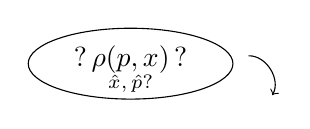
\begin{tikzpicture}
  \draw (0,0) ellipse (1.3 and 0.45);
  \node at (0,0.05) {$?\,\rho(p,x)\,?$};
  \node[font=\scriptsize] at (0,-0.25) {$\hat x,\hat p$?};
  \draw[->] (1.5,0.1) to[bend left=60] (1.8,-0.4);
\end{tikzpicture}
\end{minipage}

%----------------------------------------------------------------------
\strana{$\rho$4}
\begin{definice}[Wignerova reprezentace matice hustoty]
\begin{align*}
  \rho_W(x,p) &= \vzorec{\frac{1}{2\pi\hbar}\int_{-\infty}^{\infty}\mel{x-\tfrac12x'}{\hat\rho}{x+\tfrac12x'}\,e^{\frac{i}{\hbar}px'}\,\dd x'}
  \qquad (\text{+ zobecnění do 3D zjevné}) \\
  &= \frac{1}{2\pi\hbar}\int_{-\infty}^{\infty}\mel{p-\tfrac12p'}{\hat\rho}{p+\tfrac12p'}\,e^{-\frac{i}{\hbar}xp'}\,\dd p'
\end{align*}
\end{definice}

\underline{vlastnosti:}
\begin{itemize}[nosep]
  \item jako v klas.\ mech.: \quad $\rho(x) = \int\rho(x,p)\,\dd p$, \quad $\rho(p) = \int\rho(x,p)\,\dd x$
  \item $\operatorname{Tr}\hat\rho = \iint\rho_W(x,p)\,\dd x\,\dd p$
\end{itemize}

+ lze def.\ Wigner.\ reprezentaci měřitelných veličin
\[
  A_W(x,p) \equiv \int_{-\infty}^{\infty}\mel{x-\tfrac12x'}{\hat A}{x+\tfrac12x'}\,e^{\frac{i}{\hbar}px'}\,\dd x'
\]
\pozn{v originále $e^{-\frac{i}{\hbar}px'}$; aby platilo $\langle A\rangle = \iint\rho_WA_W$, musí mít exponent stejné znaménko jako v definici $\rho_W$ (tak i Ballentine)}

\begin{priklad}[Příklad]
\begin{tabular}{@{}lll}
potenciální energie & $V(x)\delta(x-x')$ & $\longrightarrow\ V_W(x,p) = V(x)$ \\[2pt]
kinetická energie & $\frac{p^2}{2m}\delta(p-p')$ & $\longrightarrow\ K_W = \frac{p^2}{2m}$
\end{tabular}
\end{priklad}

\begin{itemize}
  \item platí \quad $\vzorec{\langle A\rangle \equiv \operatorname{Tr}\{\rho A\} = \iint\rho_W(x,p)\,A_W(x,p)\,\dd x\,\dd p}$ \quad jako klas.\ mech.
\end{itemize}

\pozor{pozor:} $\rho(x,p)$ není pravd.\ rozdělení, protože \pozor{\underline{MŮŽE BÝT ZÁPORNÉ!}} \\
navíc není možné vytvořit úzký peak

Dá se totiž dokázat (Ballentine): \quad $\iint\rho_W(x,p)^2\,\dd x\,\dd p \leq \dfrac{1}{2\pi\hbar}$ \\
\quad tj.\ $\rho$ se supp$(\rho)$ nad \sout{objemem} oblastí $A$ \dots\ normování $\to \rho = \frac1A$ \quad $\hookrightarrow\ \Rightarrow\ A\geq 2\pi\hbar$

\begin{priklad}[PŘ: Gaussův balík]
\[
  \psi(x) = \frac{1}{\sqrt[4]{2\pi a^2}}\,e^{-x^2/4a^2} \quad\dots\ \text{Gauss balík šířky } \Delta x = a;\ \ \Delta p = \frac{\hbar}{2a}
\]
\[
  \longrightarrow\quad \rho_W(x,p) = \frac{1}{\pi\hbar}\,e^{-x^2/2\Delta x^2}\,e^{-p^2/2\Delta p^2}
\]
pro \quad $\psi(x) = \dfrac{1}{\sqrt[4]{2\pi a^2}}\,e^{-(x-x_0)^2/4a^2}\,e^{ip_0x/\hbar}$ \quad $\longrightarrow$ \quad
$\vzorec{\rho_W = \dfrac{1}{\pi\hbar}\,e^{-\frac{(x-x_0)^2}{2\Delta x^2}}\,e^{-\frac{(p-p_0)^2}{2\Delta p^2}}}$
\end{priklad}

\underline{Interference:} \quad 2 balíky centrované v $x = \pm c$

\begin{center}
\begin{tikzpicture}[gray,scale=0.9]
  \draw[->] (-4.2,0) -- (4.4,0) node[right] {$x$};
  \draw[->] (0,-1.6) -- (0,1.8) node[right] {$p$};
  % levý a pravý balík
  \foreach \c/\l in {-2.8/{-c},2.8/{+c}} {
    \draw[pattern=north east lines,pattern color=gray!40] (\c,0) ellipse (0.9 and 0.65);
    \node[black,font=\small] at (\c-0.3,0.3) {$+$}; \node[black,font=\small] at (\c+0.3,0.3) {$+$};
    \node[black,font=\small] at (\c-0.3,-0.25) {$+$}; \node[black,font=\small] at (\c+0.3,-0.25) {$+$};
    \node[font=\scriptsize] at (\c,-0.45) {$\l$};
  }
  % prostřední interferenční člen
  \draw (0,0) ellipse (0.9 and 0.65);
  \foreach \y/\s in {0.45/+,0.25/-,0.05/+,-0.15/-,-0.35/+} {
    \draw[gray!60] (-0.85,\y-0.1) -- (0.85,\y-0.1);
    \node[black,font=\tiny] at (-0.45,\y) {$\s$}; \node[black,font=\tiny] at (0.45,\y) {$\s$};
  }
  \draw[<-] (0.3,0.7) -- (1.6,1.5) node[right,font=\small] {oscilace dané faktorem $\cos\frac{2cp}{\hbar}$, amplituda konst};
  % šířky
  \draw[<->] (4.0,-0.6) -- (4.0,0.6) node[midway,right,font=\scriptsize] {$\Delta p$};
  \draw[<->] (1.9,-1.1) -- (3.7,-1.1) node[midway,below,font=\scriptsize] {$\Delta x$};
\end{tikzpicture}
\end{center}
\pozn{oscilace se rozmyjí v lim.\ $\hbar\to 0$ (ale rychleji oscilují)}

\kw{Řešení} \dots\ \kw{Husimiho distribuce} \dots\ průměrování přes min.\ plochu (Gauss)
\[
  \rho_H(x,p) = \mel{xp}{\hat\rho}{xp} \geq 0 \quad\text{ale neplatí } \rho(x) = \int\rho(x,p)\,\dd p
\]

\begin{veta}[Čas.\ vývoj (pro Wignera)]
dá se dk:
\[
  \pdv{t}\rho_W(x,p,t) = -\frac{p}{m}\pdv{x}\rho_W(x,p,t) + \dv{V}{x}\pdv{p}\rho_W(x,p,t) + \mathcal{O}(\hbar^2)
\]
\dots\ klasická \kw{Liouvilleova rovnice}
\end{veta}

%----------------------------------------------------------------------
\strana{$\rho$5}
\subsection{Matice hustoty pro složený a redukovaný systém (otevřené systémy)}

složený systém \quad $\mathcal{H} = \mathcal{H}_1\otimes\mathcal{H}_2$ \quad \dots\ báze $\ket{m_1}\ket{m_2}$

stopa operátoru \quad $\operatorname{Tr}\hat\rho \equiv \sum_{m_1m_2}\bra{m_1}\bra{m_2}\hat\rho\ket{m_1}\ket{m_2} \equiv \sum_{m_1m_2}\hat\rho_{m_1m_2,m_1m_2}$

uvažujme operátor na $\mathcal{H}_1$: \quad $\hat A_1 \equiv \hat A_1\otimes\hat I$

potom
\begin{align*}
  \langle A_1\rangle = \operatorname{Tr}\hat A_1\hat\rho
  &= \sum_{\substack{m_1m_2\\ m_1'm_2'}}\mel{m_1}{\hat A_1}{m_1'}\underbrace{\braket{m_2}{m_2'}}_{\delta_{m_2m_2'}}\bra{m_1'}\bra{m_2'}\hat\rho\ket{m_1}\ket{m_2} \\
  &= \sum_{m_1m_1'}\mel{m_1}{A_1}{m_1'}\,\rho^{(1)}_{m_1'm_1} \equiv \vzorec{\operatorname{Tr}_1\hat A_1\hat\rho^{(1)}} \quad\dots\ \text{\kw{částečná stopa}}
\end{align*}

\begin{definice}[Redukovaná matice hustoty]
\[
  \rho^{(1)}_{m_1'm_1} \equiv \sum_{m_2}\bra{m_1'}\bra{m_2}\hat\rho\ket{m_1}\ket{m_2} \equiv \mel{m_1'}{\operatorname{Tr}_2\hat\rho}{m_1}
\]
$=$ \kw{redukovaná matice hustoty}
\end{definice}

\underline{poznámky:}
\begin{itemize}
  \item všechna měření operátory působícími na $\mathcal{H}_1$ lze předpovědět jen pomocí $\hat\rho^{(1)}$. Tj.\ informace skrovná \sout{v} zbytku není důležitá pro popis systému 1 \\
        \pozn{nejde udělat se stavy -- redukce $\ket{\psi}_{12}\to\ket{\psi^{(1)}}$}
  \item $\hat\rho^{(1)}$ splňuje $\forall$ vlast.\ matice hustoty, tj.\ $\rho^\dagger = \rho$; $\mel{u}{\rho}{u}\geq 0$; $\operatorname{Tr}\rho = 1$
  \item speciální případ \dots\ nezávislé systémy \ $\hat\rho = \hat\rho_1\otimes\hat\rho_2$ \\
        pak \quad $\hat\rho^{(1)} \equiv \operatorname{Tr}_2\hat\rho = \hat\rho_1$ \quad a \quad $\hat\rho^{(2)} \equiv \operatorname{Tr}_1\hat\rho = \hat\rho_2$
  \item \pozor{$\hat\rho^{(1)}$ může být smíšený stav i v případě, že $\hat\rho$ je čistý} \\
        $\to$ model měření \dots\ přednáška Pavla Krtouše o interpretacích
  \item je možné napsat časový vývoj $\hat\rho^{(1)}$, ale pro netriviální interakci je potřeba použít aproximace \dots\ \kw{Mistrovské rovnice} \\
        $=$ vliv prostředí, dekoherence, disipace, relaxace
\end{itemize}

\begin{priklad}[PŘ: tlumený kvantový LHO]
\[
  \frac{\partial\hat\rho^{(1)}}{\partial t} =
  \underbrace{-\frac{i}{\hbar}\big[\hbar\omega a^\dagger a,\ \hat\rho^{(1)}\big]}_{\text{izolovaný LHO}}
  + \frac{\gamma}{2}\Big([a\hat\rho^{(1)}, a^\dagger] + [a, \hat\rho^{(1)}a^\dagger]\Big)
\]
\hspace*{6.8cm} $\uparrow$ malá konst.\ popisující vliv prostředí \\
\pozn{v originále první člen zapsán jako $-i\hbar[\omega a^\dagger a,\hat\rho^{(1)}]$; z $i\hbar\,\partial_t\rho = [H,\rho]$ s $H = \hbar\omega a^\dagger a$ plyne $-i\omega[a^\dagger a,\rho]$}
\end{priklad}

%----------------------------------------------------------------------
\strana{$\rho$6}
\subsection*{Řešený příklad: \ $\mathcal{H} = \mathcal{H}_{\text{spin}}\otimes\mathcal{H}_{\text{poloha}}$}
model měření spinu

\begin{center}
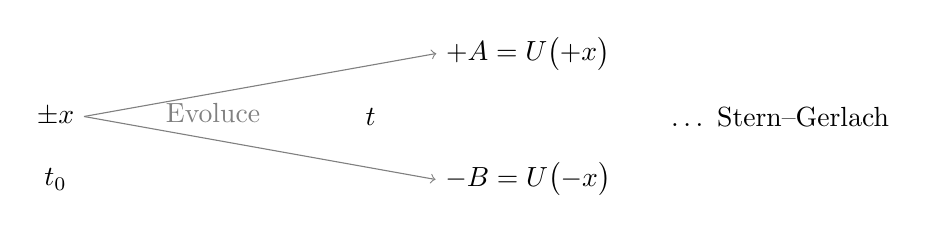
\begin{tikzpicture}
  \node (s) at (0,0) {$\ket{\pm}\ket{x}$};
  \node at (0,-0.8) {$t_0$};
  \node (a) at (6,0.8) {$\ket{+}\ket{A} = U\big(\ket{+}\ket{x}\big)$};
  \node (b) at (6,-0.8) {$\ket{-}\ket{B} = U\big(\ket{-}\ket{x}\big)$};
  \node at (4,0) {$t$};
  \draw[gray,->] (s.east) -- (a.west);
  \draw[gray,->] (s.east) -- (b.west);
  \node[gray] at (2,0.05) {Evoluce};
  \node at (9.2,0) {\dots\ Stern--Gerlach};
\end{tikzpicture}
\end{center}
Evoluce neovlivňuje spin, ale koreluje jej s polohou.

\renewcommand{\arraystretch}{1.25}
\begin{tabular}{@{}p{0.47\linewidth}@{\quad$\longrightarrow$\quad}p{0.44\linewidth}@{}}
\textcircled{1} \ $t_0$ -- čistý stav & čistý stav \\
$\ket{\psi_0} = \ket{+}\ket{x}$ \dots\ $\rho = \ket{+x}\bra{+x}$, \ $\rho_s = \ket{+}\bra{+}$ &
$\ket{\psi} = \ket{+}\ket{A}$, \quad $\rho = \ket{+A}\bra{+A}$, \ $\rho_s = \ket{+}\bra{+}$ \\
$\langle S_z\rangle = \frac{\hbar}{2}$, \ $\langle S_x\rangle = 0$ & $\langle S_z\rangle = \frac{\hbar}{2}$, \ $\langle S_x\rangle = 0$ \\
$p_+ = 1$, \ $p_{+x} = \big|\tfrac{1}{\sqrt2}(\bra{+}+\bra{-})\cdot\ket{+}\big|^2 = \frac12$ & \\[6pt]
\textcircled{2} \ nepolarizovaný stav & nepolariz.\ stav \\
stat.\ soubor: $\ket{+x}\dots\frac12$; \ $\ket{-x}\dots\frac12$ & $\ket{+A}\dots\frac12$, \quad $\ket{-B}\dots\frac12$ \\
$\to\rho = \frac12\big(\ket{+x}\bra{+x} + \ket{-x}\bra{-x}\big)$, \ $\rho_s = \frac12\hat I$ &
$\rho = \frac12\big(\ket{+A}\bra{+A} + \ket{-B}\bra{-B}\big)$ \\
$\langle S_z\rangle = 0$, \ $\langle S_x\rangle = 0$, \ $p_+ = \frac12$, \ $p_{+x} = \frac12$ & $\rho_s = \frac12\hat I$ \dots\ měření jako $t_0$ \\[6pt]
\textcircled{3} \ čistý stav & čistý stav \\
$\ket{\psi_0} = \tfrac{1}{\sqrt2}\big(\ket{+x} + \ket{-x}\big)$ \dots\ vl.\ st.\ $S_x\dots +\frac{\hbar}{2}$ &
$\ket{\psi} = \tfrac{1}{\sqrt2}\big(\ket{+A} + \ket{-B}\big)$ \\
$\to\rho = \frac12\big(\ket{+x}\bra{+x} + \ket{-x}\bra{-x} + \ket{+x}\bra{-x} + \ket{-x}\bra{+x}\big)$ &
$\rho = \frac12\big(\ket{+A}\bra{+A} + \ket{-B}\bra{-B} + \ket{+A}\bra{-B} + \ket{-B}\bra{+A}\big)$ \\
$\rho_s = \frac12\begin{pmatrix}1&1\\1&1\end{pmatrix}$ &
$\rho_s = \frac12\begin{pmatrix}1&0\\0&1\end{pmatrix} = \frac12 I$ \dots\ \pozor{redukce jako po měření $S_z$!} \\
$\langle S_z\rangle = 0$, \ $\langle S_x\rangle = \frac{\hbar}{2}$, \ $p_+ = \frac12$, \ $p_{+x} = 1$ &
$\langle S_z\rangle = 0$, \ $\langle S_x\rangle = 0$, \ $p_+ = \frac12$, \ $p_{+x} = \frac12$ \\[6pt]
\textcircled{4} \ nepolarizovaný stav & nepolariz.\ stav \\
$\ket{\psi_0} = \tfrac{1}{\sqrt2}\big(\ket{+x} + \ket{-x}\big)$; \ $\tfrac{1}{\sqrt2}\big(\ket{+x} - \ket{-x}\big)$, \ $p = \frac12$, $p = \frac12$ &
$\tfrac{1}{\sqrt2}\big(\ket{+A} + \ket{-B}\big)$, \ $\tfrac{1}{\sqrt2}\big(\ket{+A} - \ket{-B}\big)$, \ $p = \frac12$, $p = \frac12$ \\
$\rho = \frac12\big(\ket{+x}\bra{+x} + \ket{-x}\bra{-x}\big)$ \dots\ $\rho_s = \frac12\hat I$ &
$\rho = \frac12\big(\ket{+A}\bra{+A} + \ket{-B}\bra{-B}\big)$, \ $\rho_s = \frac12\hat I$ \\
$\langle S_z\rangle = \langle S_x\rangle = 0$, \ $p_+ = p_{+x} = \frac12$ & $\langle S_z\rangle = \langle S_x\rangle = 0$, \ $p_+ = p_{+x} = \frac12$
\end{tabular}
\renewcommand{\arraystretch}{1}

\dots\ udělat na cvičení!

\noindent\rule{\linewidth}{0.4pt}

\begin{priklad}[PŘ 2]
nechť $H = H_1 + H_2$, kde $H_1$ působí na $\mathcal{H}_1$ a $H_2$ na $\mathcal{H}_2$ \dots\ $\mathcal{H} = \mathcal{H}_1\otimes\mathcal{H}_2$ \\
napište evoluční rovnici pro redukovanou matici hustoty \hfill \textcolor{Red}{$\nwarrow$ separované systémy} \\
\phantom{x} \hfill \textcolor{Red}{$\to$ nezávislá dynamika}
\[
  \operatorname{Tr}_2\Big(i\hbar\frac{\partial\rho}{\partial t} = [H,\rho]\Big)
\]
\[
  \hookrightarrow\quad i\hbar\pdv{t}\rho^{(1)} = \underbrace{\operatorname{Tr}_2(H_1\rho - \rho H_1)}_{[H_1,\rho^{(1)}] = H_1\rho^{(1)} - \rho^{(1)}H_1}
  + \underbrace{\operatorname{Tr}_2(H_2\rho - \rho H_2)}_{0\ \leftarrow\ \text{DK: rozpis do bází}}
\]
\end{priklad}

